\documentclass[11pt]{article}

% -- Color scheme
\usepackage{xcolor}

% Default colors
\definecolor{minimal-main}{HTML}{131313}
\definecolor{minimal-light}{HTML}{F2F2F2}
\definecolor{minimal-contrast}{HTML}{F3F2F5}

% Additional color definitions
\definecolor{minimal-black}{HTML}{131313}
\definecolor{minimal-white}{HTML}{F3F2F5}
\definecolor{minimal-red}{HTML}{C43C2D}
\definecolor{minimal-blue}{HTML}{343454}
\definecolor{minimal-yellow}{HTML}{F1C40F}
\definecolor{minimal-green}{HTML}{2D6514}
\definecolor{minimal-beige}{HTML}{D7B6A5}

% Colorbox environments
\usepackage[most]{tcolorbox}

% -- Page layout
\usepackage[paperheight=842pt, paperwidth=595pt, margin=0pt]{geometry}
\setlength{\parindent}{0pt}

% Interline spacing options
\newcommand{\largespace}{\\[2pt]}
\newcommand{\mediumspace}{\\[-3pt]}
\newcommand{\smallspace}{\\[-5pt]}

% In-box spacing around content
\newcommand{\inboxspacing}{.015\paperheight}

% Horizontal spacing of the boxes (must sum up to 1)
\newcommand{\sideboxwidth}{.35}
\newcommand{\mainboxwidth}{.65}

% Vertical spacing of the boxes (must sum up to 1)
\newcommand{\headboxheight}{.080}
\newcommand{\mainboxheight}{.910}
\newcommand{\footboxheight}{.010}

% -- Font settings
\usepackage[letterspace=20]{microtype}
\usepackage[T1]{fontenc}
\usepackage{raleway}
\renewcommand{\familydefault}{\sfdefault}

% Custom font commands
\newcommand{\header}[1]{\uppercase{\textbf{\fontsize{30}{100}{\lsstyle{#1}}}}}
\newcommand{\titlefont}[1]{\uppercase{\textbf{\Large{#1}}}}

% -- Additional packages
\usepackage{multirow}
\usepackage{array}
\usepackage{tikz}
\usepackage{hyperref}
\urlstyle{same}

\begin{document}

\begin{tcbposter}[
    poster = {columns=1, rows=1, spacing=0pt},
    boxes = {sharp corners, halign=center, valign=center, boxrule=0pt}
]

% -- Headbox
\posterbox[
    colback=minimal-main,
    halign=center]
    {name=headbox,
    span=1,
    rowspan=\headboxheight}
{
    \color{white}
    \header{{{name}}}
    
    \vspace{-7px}
    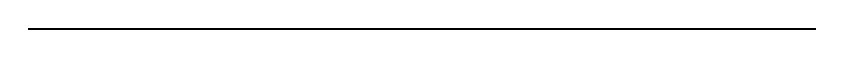
\begin{tikzpicture}
        \draw[fill=white] (-5.0, -0.01) rectangle (5.0, 0.01);
    \end{tikzpicture}
    \vspace{5px}
    
    \titlefont{{{summary}}}
}

% -- Sidebox
\posterbox[
    colback=minimal-light,
    valign=top,
    top=\inboxspacing,
    halign=right,
    right=\inboxspacing]
    {name=sidebar,
    below=headbox,
    column=1,
    span=\sideboxwidth,
    rowspan=\mainboxheight}
{
    \begin{tabular}{rl}
        \multicolumn{2}{@{}c@{}}{\scalebox{0.25}{\input{{{image}}}}} \\
        \mediumspace
        & \titlefont{Contact} \\
        
        \hline \mediumspace
        {{contact_info}}
        
        & \titlefont{Personal} \\
        \hline \mediumspace
        
        {{personal_info}}
        
        & \titlefont{Platforms} \\
        \hline \mediumspace
        
        {{platforms}}
        
        & \titlefont{Languages} \\
        \hline \mediumspace
        
        {{languages}}
    \end{tabular}
}

% -- Mainbox
\posterbox[
    colback=white,
    valign=top,
    top=\inboxspacing,
    halign=left,
    left=\inboxspacing  ]
    {name=mainbox,
    column*=1,
    span=\mainboxwidth,
    below=headbox,
    rowspan=\mainboxheight}
{
    \begin{tabular}{>{\footnotesize}rl}
        & \titlefont{About Me} \\
        \hline \mediumspace
        
        {{about}}\\
        & \titlefont{Education} \\
        \hline \mediumspace
        
        {{education}}
        
        & \titlefont{Work Experience} \\
        \hline \mediumspace
        
        {{work_experience}}
        
        & \titlefont{Selected Publications} \\
        \hline \mediumspace
        
        {{publications}}
        
        & \titlefont{Awards} \\
        \hline \mediumspace
        
        {{awards}}
        

        
        & \titlefont{Skills} \\
        \hline \mediumspace
        
        {{skills}}
    \end{tabular}
}

% -- Footbox
\posterbox[colback=minimal-main]
           {name=blankbox2,
           below=sidebar,
           column=1,
           span=1,
           rowspan=\footboxheight}{}

\end{tcbposter}

\end{document}